\documentclass[10pt,a4paper]{article}
\usepackage[margin=2.3cm]{geometry}
\usepackage[T1]{fontenc}
\usepackage{lmodern,microtype,booktabs,graphicx,float,xcolor,caption,enumitem,array,amsmath}
\usepackage[colorlinks=true,linkcolor=blue!50!black,urlcolor=blue!50!black]{hyperref}
\captionsetup{font=small,labelfont=bf}
\setlist{itemsep=1pt,topsep=3pt}
\renewcommand{\arraystretch}{1.1}
\newcommand{\auc}{AUROC}
\title{\textbf{Cross-corpus and Multimodal Tuberculosis Detection:\\Toward Model Generalization}\\[4pt]\large Experiment report}
\author{Bagus Tris Atmaja\\\small \texttt{multibench} repository, \texttt{datasets/tb\_multi}}
\date{4 November 2026 (revised)}
\begin{document}
\maketitle
\begin{abstract}\noindent
Chest X-ray (CXR) classifiers for tuberculosis (TB) often look excellent in-distribution and fail on a new site. We build a six-corpus benchmark (Qatar, Montgomery, Shenzhen, TBX11K, Pakistan/Mendeley, and the multimodal CIDRZ/Google Health AI cohort), add VinDr-CXR (radiologist-labelled, 646 TB-positive images) as a second external cohort, audit them for duplicates and shortcuts, and evaluate generalization with leave-one-corpus-out (LOCO) fine-tuning of several backbones and domain-generalization (DG) methods. We then test whether the best image expert improves multimodal (text + audio + CXR) detection on CIDRZ, an external target never used for model selection.
Main findings (five seeds, per-backbone tuning on the public folds only): (i) corpus identity alone predicts the TB label (pooled AUROC 0.83) and silhouette- or border-only controls reach AUROC up to 0.84; artefact-only predictors reach 0.85--1.00 within-corpus on Qatar, TBX11K and Pakistan, and Pakistan is not identifiable (artefact-only AUROC 1.000); (ii) lung masking plus strong augmentation, and above all a CXR foundation model (RAD-DINO, LOCO mean AUROC 0.898 vs 0.867 for tuned ImageNet ViT-B/16), improve generalization on the public corpora, whereas classical DG losses do not beat source-balanced sampling; (iii) on the external CIDRZ cohort every backbone sits at AUROC 0.77--0.81 with overlapping CIs, and artefact-stratified AUROC stays within 0.01 of raw (0.816 vs 0.825 for RAD-DINO); late fusion lifts text from 0.782 to 0.85 and audio adds nothing; (iv) probabilities are badly miscalibrated across sites (ECE up to 0.49) and local Platt recalibration repairs calibration (ECE 0.07) but not discrimination: no model meets the WHO triage profile (sensitivity $\ge$90\%, specificity $\ge$70\%) on CIDRZ even with an oracle threshold; (v) on the larger VinDr-CXR cohort the foundation-model advantage is confirmed (weighted AUROC 0.903 for RAD-DINO vs 0.870 for tuned ViT, paired difference $+0.032$ [0.018, 0.049], RAD-DINO+MixStyle 0.917), the artefact-stratified AUROC stays within 0.02 of raw (0.899 vs 0.919), and an oracle threshold reaches the WHO profile for RAD-DINO (sensitivity 0.91 at 70\% specificity) but a deployable threshold does not, with the caveat that VinDr's reference standard is radiologist reading, not microbiology.
\paragraph{Revision note.} This version supersedes the first one: a checkpoint-restore bug (only parameters named ``vit.encoder''/``head'' were restored at the best epoch, leaving CNN tails and RAD-DINO's final layer-norm at last-epoch values) affected the ResNet50, xrv-DenseNet and RAD-DINO runs. All headline numbers were re-run after the fix with five seeds; the earlier RAD-DINO LOCO mean 0.906 is now 0.898 (tuned), ResNet50 0.786 $\rightarrow$ 0.816, xrv-DenseNet 0.784 $\rightarrow$ 0.809, and the fusion and calibration results were recomputed with corrected experts.
\paragraph{Revision note 2.} VinDr-CXR was added as a second external cohort (Section~\ref{sec:vindr}): same eight tuned configurations, five seeds, trained on the four public sources only, with weighted metrics because the evaluation sample is enriched for TB.
\paragraph{Revision note 3.} Material that was in the accompanying slide deck but not in this report was added: example images and the lung-mask illustration, the fold layout, the shortcut-control table, a backbone table, one-line descriptions of the DG methods, worked examples for artefact-adjusted AUROC, ECE and Platt scaling, a bootstrap of the CIDRZ oracle operating points (Section~\ref{sec:why-cidrz}), next steps, and a glossary (Appendix~\ref{app:glossary}).\end{abstract}

\section{Introduction and goals}
The study asks which methods improve (a) cross-corpus generalization of CXR TB detection and (b) multimodal fusion. It extends earlier work on Qatar $\rightarrow$ CIDRZ transfer, where lung masking raised CIDRZ zero-shot AUROC of a small VGG from $0.613\pm0.049$ to $0.729\pm0.011$ (seed-average difference $+0.125$, 95\% CI $[+0.030,+0.217]$) by removing non-lung cues such as anonymization boxes present in about 30\% of Qatar TB images versus under 1\% of normals. Here that finding is generalized to four public source corpora with a principled protocol.

\paragraph{Protocol.} \emph{Leave-one-corpus-out:} train on the three other source corpora (plus validation from the held-in corpora), test on the held-out one. For the CIDRZ target all four source corpora are pooled. CIDRZ is never used for method or hyper-parameter selection; hyper-parameters were chosen per backbone on the four public folds only (pre-declared rule, Section~\ref{sec:tuning}). Metric: AUROC with paired-bootstrap 95\% confidence intervals on seed-averaged scores; five seeds per cell for the headline comparison (two seeds for the DG-loss exploration and the 448\,px arm).

\begin{table}[H]\centering\small
\begin{tabular}{lcccc|c}\toprule
Fold & Qatar & NLM & TBX11K & Pakistan & CIDRZ, VinDr-CXR\\\midrule
1 & \textbf{test} & train & train & train & external\\
2 & train & \textbf{test} & train & train & external\\
3 & train & train & \textbf{test} & train & external\\
4 & train & train & train & \textbf{test} & external\\
external & train & train & train & train & \textbf{test}\\\bottomrule
\end{tabular}\caption{Leave-one-corpus-out layout. Random splits would hide the problem, because images from the same hospital then sit in both train and test; LOCO forces the model to face a site it has never seen. Method selection used only folds 1--4.}\end{table}

\section{Data}
All images are standardized to $224\times224$ uint8 (per-corpus arrays and metadata under \texttt{data/tb\_multi}). TBX11K is restricted to active TB versus healthy and sick-non-TB; latent and uncertain cases are excluded.
\begin{table}[H]\centering\small
\begin{tabular}{lrr>{\raggedright\arraybackslash}p{3.3cm}}\toprule
Corpus & $n$ (after dedup) & TB prevalence & Notes\\\midrule
Qatar & 4187 & 16.4\% & large public CXR set\\
NLM (Montgomery+Shenzhen) & 138+661 = 799 & 49\% & two US/China screening sets merged\\
TBX11K & 8029 & 8.2\% & lesion bounding boxes available\\
Pakistan (Mendeley v3) & 2973 & 82.9\% & $\sim$256\,px JPEG, TB-dominant\\
CIDRZ / Google Health AI & 364 & 16.5\% (60 pos.) & text + audio + CXR; external target\\
VinDr-CXR (PhysioNet) & 2146 sampled & 30.1\% in sample (3.6\% weighted) & radiologist labels; external target (Section~\ref{sec:vindr})\\\bottomrule
\end{tabular}\caption{Corpora used. Dedup counts follow Section~\ref{sec:dedup}.}\end{table}
\begin{figure}[H]\centering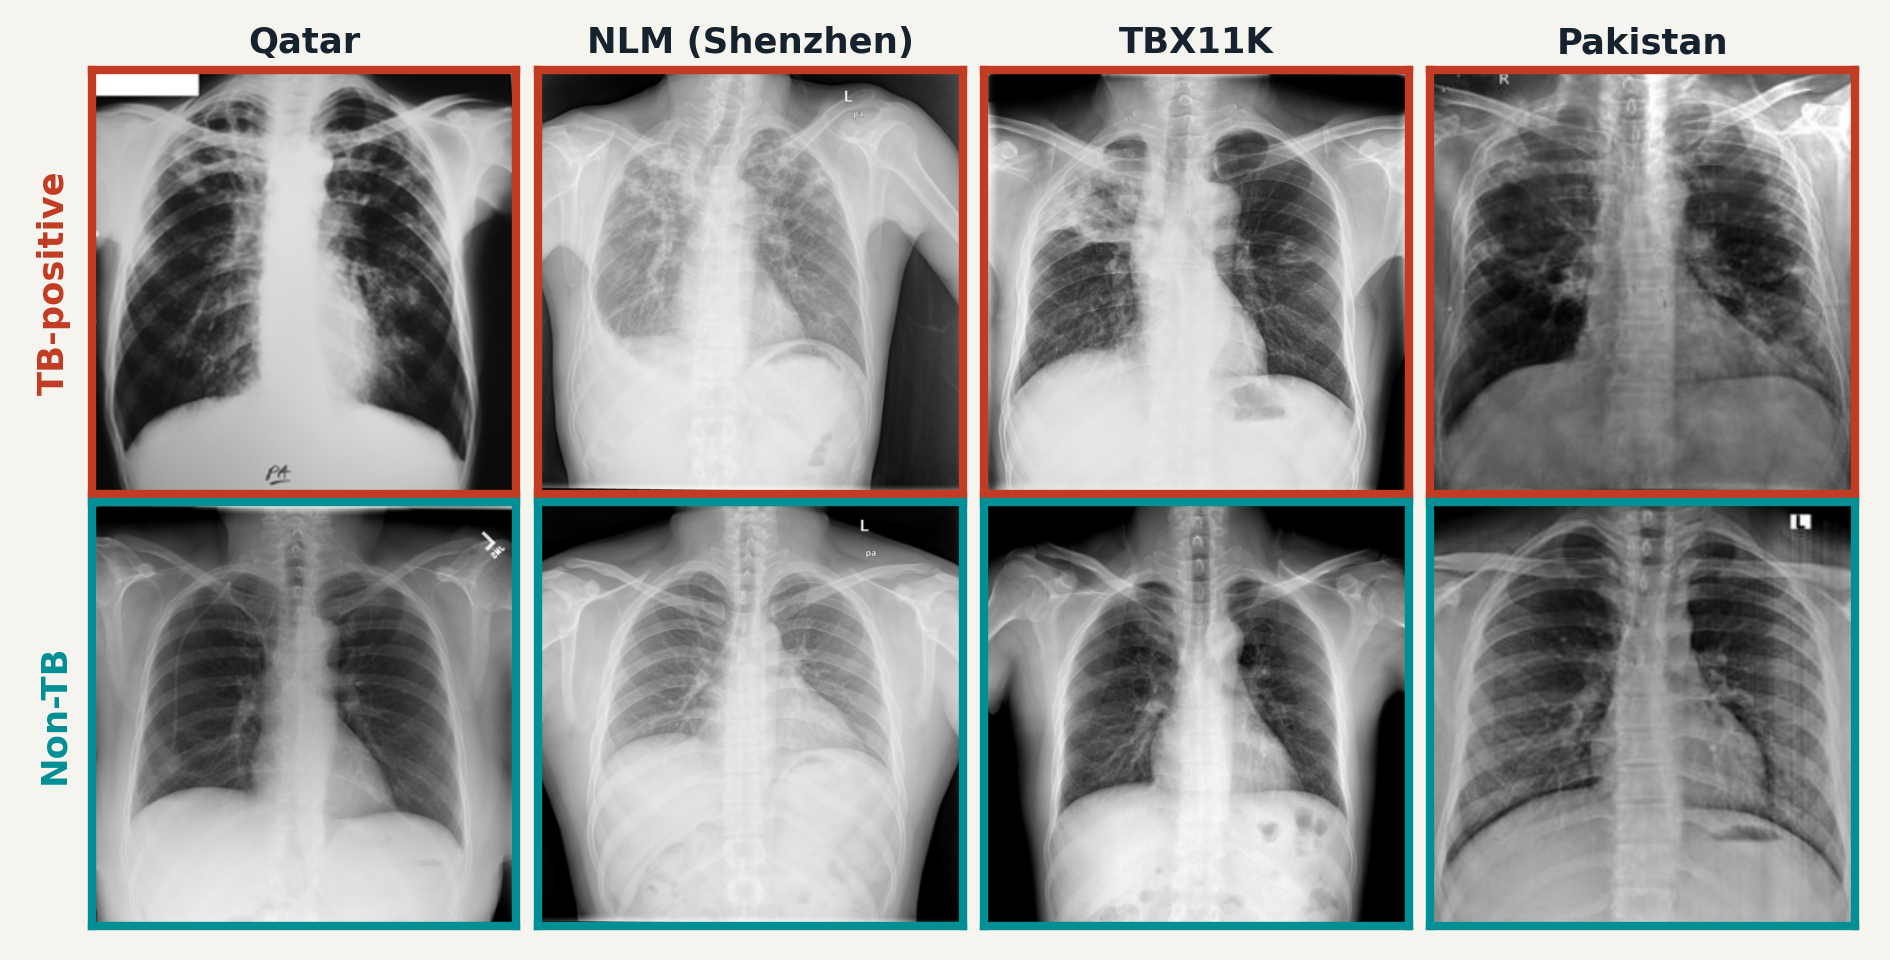
\includegraphics[width=.95\linewidth]{fig_xray_examples.png}
\caption{One TB-positive (top row, red frame) and one non-TB (bottom row, teal frame) chest X-ray per public corpus. The images are typical rather than extreme cases: they sit at the 75th percentile of RAD-DINO's held-out score among positives and the 25th among negatives. TB signs here include upper-lobe opacities, cavities and scarring, and are often subtle. Scanners, contrast, borders and markers differ clearly between corpora, which is why a model can learn the corpus rather than the disease; note the white anonymization box on the Qatar TB image (such boxes occur in about 30\% of Qatar TB images and under 1\% of normals). Non-TB in TBX11K includes sick patients without TB; non-TB in Pakistan is labelled ``other''.}\label{fig:xray}\end{figure}

\section{Cross-corpus duplicate check}\label{sec:dedup}
Near-duplicates across corpora would inflate LOCO scores. We combine a 64-bit DCT perceptual hash (Hamming $\le 8$) with a $64\times64$ pixel correlation ($\ge0.97$). The detector was calibrated with a positive control: TBX11K ships 400 known Montgomery/Shenzhen copies, recovered essentially 100\% (329 + 73 pairs; embedding cosine p5 $=0.997$).

The scan found 293 pairs, all within-corpus except 12 Qatar$\times$TBX11K, with no label conflicts. The drop list removed 231 TBX11K, 35 Pakistan, 13 Qatar and 1 Shenzhen images (CIDRZ is never dropped). Importantly, \emph{no} Qatar--NLM near-duplicates exist: best pixel correlation 0.948 (copies would be $\sim$1.0) and best xrv-embedding cosine 0.978 against 0.973 for a null corpus pair, confirmed visually (Figure~\ref{fig:dedup}). This contradicts an earlier assumption that Qatar's TB class pools Montgomery and Shenzhen. VinDr-CXR was checked separately against every other corpus (\texttt{dedup\_external.py}): 0 cross-corpus pairs, one within-VinDr pair with identical labels (kept), and a positive control of 105 perturbed copies of source images was recovered 105/105. Limitation: heavy crops, flips or mirroring are not covered.
\begin{figure}[H]\centering\includegraphics[width=.92\linewidth]{shenzhen_montgomery_to_qatar_top.png}
\caption{Closest Shenzhen/Montgomery $\rightarrow$ Qatar matches: different patients.}\label{fig:dedup}\end{figure}

\section{Shortcut audit}
Using frozen torchxrayvision DenseNet121 features and trivial controls: the corpus can be identified from embeddings with 96.8\% accuracy, and corpus id alone predicts the TB label with pooled 5-fold AUROC 0.831 (because prevalence ranges from 8\% to 83\%). Figure~\ref{fig:shortcut} shows that a classifier seeing only the lung silhouette, or only outer border pixels, reaches AUROC 0.84 (silhouette) and 0.78 (border) on Qatar, and 0.80 / 0.76 on Pakistan. Qatar and Pakistan held-out scores are therefore largely explainable by acquisition artefacts; they should be read with caution, and Pakistan is the least trustworthy target. TBX11K and CIDRZ are less affected (silhouette 0.60 / 0.61). On VinDr-CXR the source-trained controls give 0.62 (mask area), 0.64 (silhouette) and 0.67 (border) on the unweighted sample, and 0.72 weighted (Section~\ref{sec:vindr}).
\begin{table}[H]\centering\small
\begin{tabular}{lccccc}\toprule
Control, held-out AUROC & Qatar & NLM & TBX11K & Pakistan & CIDRZ\\\midrule
Lung silhouette only & \textbf{.84} & .71 & .60 & \textbf{.80} & .61\\
Outer border only & .78 & .53 & .61 & .76 & .46\\
Frozen X-ray probe (xrv) & .84 & .73 & .69 & .68 & .70\\\bottomrule
\end{tabular}\caption{Shortcut controls (0.5 is chance). The first two controls see no lung tissue content, only the outline of the lungs or only the outer border pixels.}\label{tab:shortcut}\end{table}
\begin{figure}[H]\centering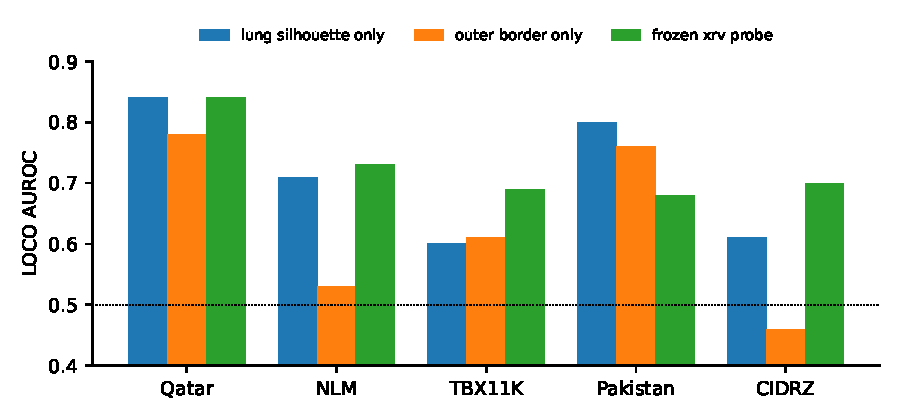
\includegraphics[width=.7\linewidth]{fig_shortcut.pdf}
\caption{LOCO AUROC of shortcut controls and of a frozen xrv probe.}\label{fig:shortcut}\end{figure}

\section{Methods}\label{sec:methods}
\paragraph{Backbones.} torchvision ViT-B/16 (ImageNet), RAD-DINO (\texttt{microsoft/rad-dino}, a CXR foundation model; 224\,px, with a 448\,px arm), ResNet50 and xrv-DenseNet121. Each backbone's learning rate and unfrozen depth were tuned on the four public LOCO folds (Section~\ref{sec:tuning}): ViT lr $10^{-4}$, 6 blocks; RAD-DINO lr $10^{-4}$, 6 blocks; ResNet50 lr $10^{-3}$, layer3+4; xrv-DenseNet lr $10^{-3}$, denseblock4. The earlier ViT DG-loss exploration used lr $5\times10^{-5}$ from a CIDRZ-informed sweep.
\begin{table}[H]\centering\small
\begin{tabular}{llll}\toprule
Backbone & Pretrained on & Selected learning rate & Unfrozen part\\\midrule
ViT-B/16 & everyday photos (ImageNet) & $10^{-4}$ & last 6 blocks\\
RAD-DINO & chest X-rays (self-supervised) & $10^{-4}$ & last 6 blocks\\
ResNet50 & everyday photos (ImageNet) & $10^{-3}$ & layer3 and layer4\\
xrv-DenseNet121 & many chest X-ray sets & $10^{-3}$ & denseblock4\\\bottomrule
\end{tabular}\caption{Backbones and their settings chosen on the four public folds (96 runs, rule fixed beforehand; CIDRZ never used).}\end{table}
\paragraph{Training recipes.} ERM; source-balanced sampling (sbal); GroupDRO; V-REx; CORAL; DANN; per-domain feature standardization (dstd); lung masking (PSPNet, lungs + hila, dilated 6\,px); strong GPU augmentation (affine, gamma/contrast, resolution jitter, border erasing); MixStyle ($p=0.5$, $\alpha=0.1$, on activations entering the trainable tail); and TBX11K lesion-box supervision (an auxiliary patch-token loss). \emph{In one line each:} \emph{source-balanced sampling} draws equal numbers from each training corpus so the largest does not dominate; \emph{MixStyle} mixes image-style (mean and variance) statistics between sites; \emph{GroupDRO} optimizes the worst-performing site; \emph{V-REx} penalizes the variance of the risk across sites; \emph{CORAL} matches feature statistics between sites; \emph{DANN} trains the model so that a site classifier cannot recognize the site; \emph{augmentation} varies shifts, contrast and resolution so the model sees varied images. None of the DG losses beat simple source-balanced sampling here.
\paragraph{Multimodal CIDRZ.} Image experts are trained without CIDRZ; text and audio models are fit within cross-validation (10$\times$ repeated 5-fold). Fusion variants: stacking, concatenation, reliability-weighted (relw), and a modality-dropout MLP (MD-MLP), evaluated with paired bootstrap and modality-missing tests.
\begin{figure}[H]\centering\includegraphics[width=.9\linewidth]{cidrz_overlay.png}
\caption{Lung-hilum masks (green) on CIDRZ examples; everything outside is set to black.}\end{figure}
\begin{figure}[H]\centering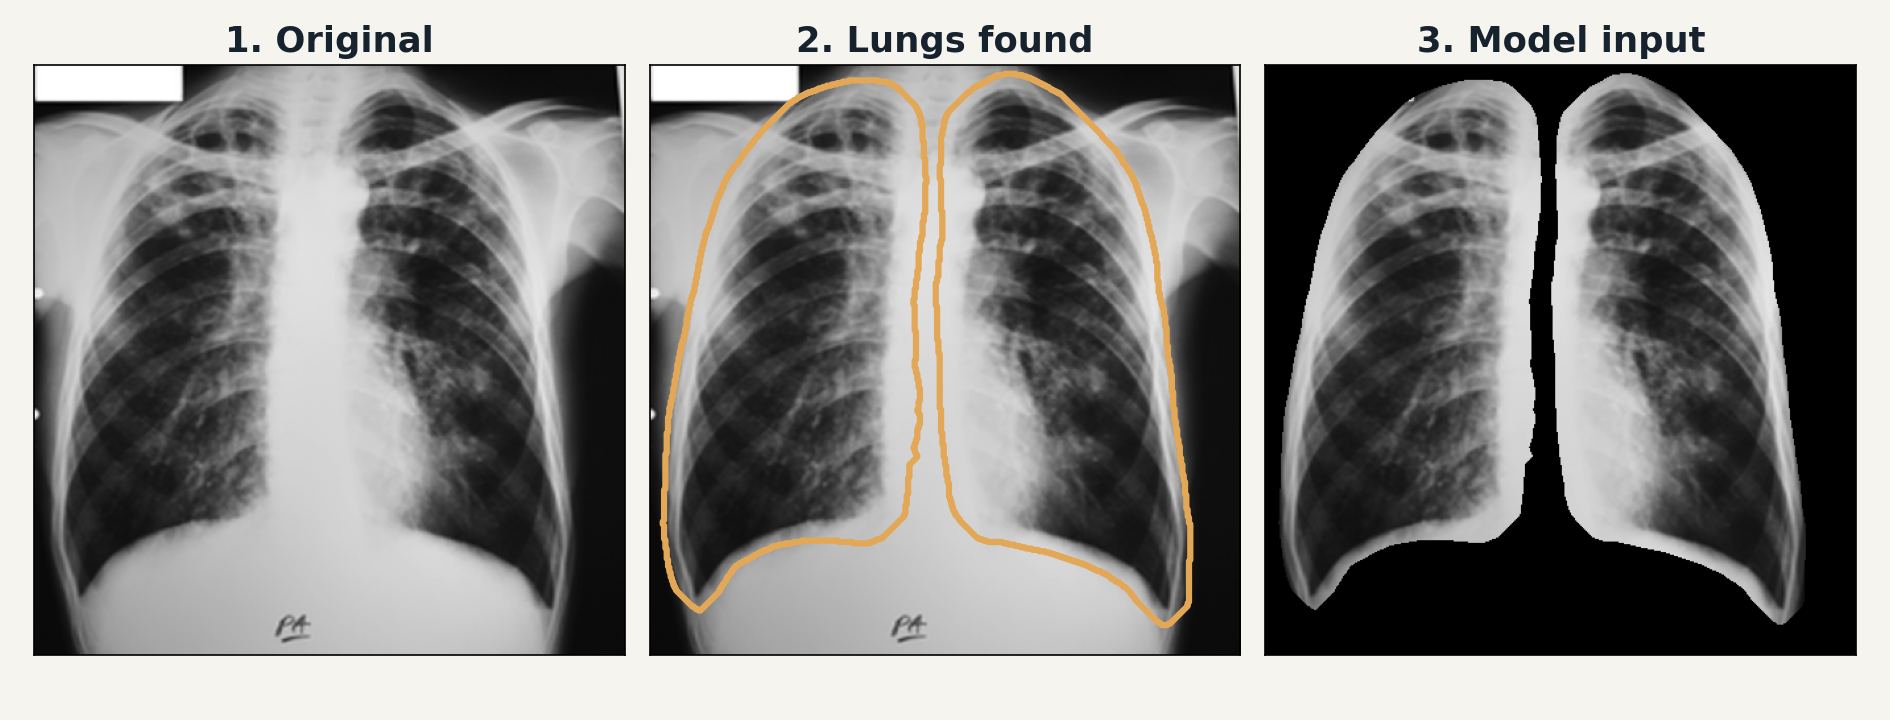
\includegraphics[width=.9\linewidth]{fig_lung_mask.png}
\caption{Lung masking on a Qatar TB image: original, lungs found by the segmentation network, and the model input. The mask is closed, filled and widened by 6 pixels at 224 px so the pleural edge stays visible; the white anonymization box and the bottom marker are removed, so the model cannot use them.}\end{figure}

\section{Tuning protocol}\label{sec:tuning}
A grid of 24 configurations per backbone family (96 runs, seed 0) was evaluated on Qatar, NLM, TBX11K and Pakistan; CIDRZ was never used. The pre-declared rule picks the best mean AUROC over the four folds and, among configurations within 0.01, the one with fewer unfrozen blocks and lower learning rate (\texttt{results/tuning\_protocol.md}). Tuning gains over the untuned configurations were small (at most $+0.034$; RAD-DINO $+0.007$), so the ranking of backbones was not changed. Selecting on NLM + TBX11K only, because Pakistan and Qatar are artefact-prone, picks different configurations for RAD-DINO, ResNet50 and xrv-DenseNet (\texttt{results/tuning\_summary.md}); we report the primary rule.

\section{Results: LOCO generalization}
\begin{figure}[H]\centering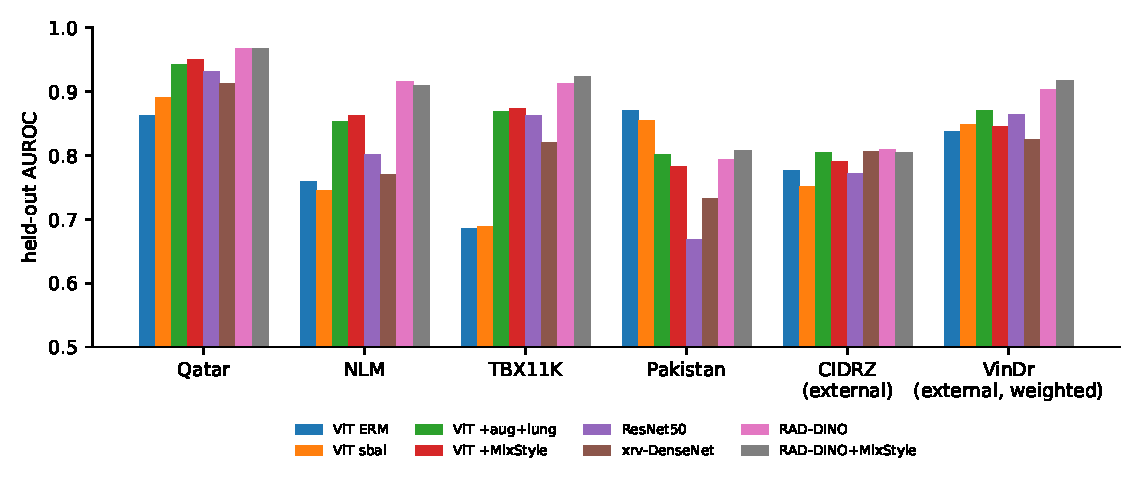
\includegraphics[width=\linewidth]{fig_loco.pdf}
\caption{Held-out AUROC, five-seed means, tuned backbones. CIDRZ and VinDr-CXR (weighted AUROC) are external.}\label{fig:loco}\end{figure}
\begin{table}[H]\centering\footnotesize
\begin{tabular}{lccccccc}\toprule
Method (5 seeds) & Qatar & NLM & TBX11K & Pakistan & CIDRZ & VinDr$^\dagger$ & LOCO mean\\\midrule
RAD-DINO + MixStyle & .967 & .909 & .923 & .808 & .805 & .917 & \textbf{.902}\\
RAD-DINO (sbal+aug+lung) & .968 & .916 & .913 & .794 & .809 & .903 & .898\\
ViT + MixStyle & .951 & .862 & .874 & .783 & .790 & .846 & .867\\
ViT (sbal+aug+lung) & .942 & .854 & .869 & .801 & .804 & .870 & .867\\
ResNet50 & .932 & .802 & .862 & .669 & .772 & .864 & .816\\
xrv-DenseNet121 & .913 & .771 & .820 & .732 & .807 & .825 & .809\\
ViT sbal, whole image, no aug & .891 & .745 & .689 & .855 & .751 & .848 & .795\\
ViT ERM, whole image & .863 & .760 & .685 & .870 & .777 & .837 & .795\\\bottomrule
\end{tabular}\caption{Final LOCO AUROC, mean of five seeds (tuned lr). Standard deviations across seeds are 0.005--0.03 on the public folds, up to 0.12 for ResNet50 on Pakistan (\texttt{results/loco\_final\_summary.md}). ``LOCO mean'' averages the four public corpora. $^\dagger$VinDr-CXR: weighted AUROC, mean of five seeds, trained on the four public sources only (Section~\ref{sec:vindr}); radiologist labels.}\label{tab:loco}\end{table}

\begin{table}[H]\centering\footnotesize
\begin{tabular}{lccccc}\toprule
vs ViT (sbal+aug+lung), paired bootstrap & Qatar & NLM & TBX11K & Pakistan & CIDRZ\\\midrule
RAD-DINO & $+.024$ & $+.067$ & $+.043$ & $-.006$ & $+.015$\\
 & {\tiny[.014,.033]} & {\tiny[.045,.090]} & {\tiny[.033,.053]} & {\tiny[$-$.021,.010]} & {\tiny[$-$.028,.060]}\\
ResNet50 & $-.003$ & $-.044$ & $-.003$ & $-.121$ & $-.020$\\
xrv-DenseNet & $-.028$ & $-.091$ & $-.052$ & $-.072$ & $+.011$\\
ViT ERM, whole image & $-.074$ & $-.094$ & $-.187$ & $+.073$ & $-.021$\\\bottomrule
\end{tabular}\caption{Seed-averaged AUROC differences against tuned ViT with 95\% CIs (RAD-DINO row; the others' CIs are in the summary file).}\end{table}
\begin{itemize}
\item \textbf{Preprocessing beats loss engineering.} Lung masking, source-balanced sampling and strong augmentation raise ViT over ERM by $+0.074$ (Qatar), $+0.094$ (NLM) and $+0.187$ (TBX11K) but lower Pakistan by $0.073$, where ERM is best (0.870). Pakistan is the artefact-dominated corpus, so a method that scores well there is not necessarily better. In the two-seed exploration, GroupDRO, V-REx, CORAL and DANN did not beat source-balanced sampling on average (LOCO means 0.78--0.81; Table~\ref{tab:dg}).
\item \textbf{A foundation backbone is the largest gain on the public corpora.} RAD-DINO beats tuned ViT on Qatar, NLM and TBX11K (CIs exclude 0), with LOCO mean 0.898 vs 0.867; ResNet50 and xrv-DenseNet are 0.05--0.09 lower.
\item \textbf{On CIDRZ no backbone is distinguishable.} All sit at 0.77--0.81 and every paired difference has a CI that includes 0. The CIDRZ interval for RAD-DINO vs ViT ([$-.028,+.060$]) includes the VinDr-sized difference; on VinDr-CXR (646 positives, Section~\ref{sec:vindr}) the advantage reappears.
\item \textbf{MixStyle} is not a reliable gain: RAD-DINO $+0.004$ mean, ViT $\pm0.00$ (Pakistan $-0.015$, CIDRZ $-0.013$).
\item \textbf{Lesion supervision} (two seeds, exploration, earlier code): no gain for the CLS score for ViT or RAD-DINO; see \texttt{results/loco\_summary\_all.md}. Not re-run.
\end{itemize}
\begin{table}[H]\centering\footnotesize
\begin{tabular}{lcccccc}\toprule
Method (ViT, 2 seeds) & Qatar & NLM & TBX11K & Pakistan & CIDRZ & LOCO mean\\\midrule
ViT sbal+aug+lung+dstd & .911 & .811 & .862 & .811 & .795 & .849\\
ViT sbal+lung & .931 & .814 & .842 & .752 & .796 & .835\\
ViT sbal+aug & .922 & .807 & .800 & .708 & .794 & .809\\
CORAL & .854 & .813 & .708 & .852 & .683 & .807\\
DANN & .798 & .765 & .740 & .898 & .712 & .800\\
V-REx & .887 & .707 & .732 & .820 & .767 & .786\\
GroupDRO & .885 & .756 & .724 & .776 & .761 & .785\\
ViT sbal (no preprocessing) & .881 & .766 & .711 & .769 & .764 & .782\\\bottomrule
\end{tabular}\caption{Earlier two-seed ViT-B/16 exploration of recipes and DG losses (lr $5\times10^{-5}$; not retuned; ViT code paths were unaffected by the checkpoint bug).}\label{tab:dg}\end{table}

\subsection*{Resolution: RAD-DINO at 448\,px}
RAD-DINO was trained on a native 448\,px cache (all corpora re-standardized from the originals, CIDRZ from its DICOMs; two seeds, same tuned configuration). Resolution was checked after the artefact audit on purpose: a gain on public folds alone says nothing about transfer.
\begin{table}[H]\centering\small
\begin{tabular}{lccc}\toprule
RAD-DINO AUROC & 224\,px & 448\,px & Change\\\midrule
Qatar & .965 & .971 & $+.006$\\
NLM & .917 & .951 & $+.034$\\
TBX11K & .907 & .946 & $+.039$\\
Pakistan & .815 & .932 & $+.117$\\
CIDRZ (external) & .820 & .824 & $+.004$\\\bottomrule
\end{tabular}\caption{RAD-DINO at 224 vs 448\,px (two seeds).}\end{table}
Resolution helps on the public folds but gives no external gain; the large Pakistan jump cannot be attributed to pathology given that corpus's artefact structure, and we do not treat it as evidence of better transfer.

\section{Artefact-adjusted AUROC}
Because artefacts predict labels within corpora, we stratify target cases and controls by predicted-artefact score (silhouette, border and area features; \texttt{datasets/tb\_multi/artefact\_adjust.py}) and average AUROC within strata, with the artefact predictor fit either on the source corpora (src) or by cross-validation within the target (cv; strongest control). \paragraph{Worked example (illustrative numbers, not our data).} Cut the artefact score into three bins. A ``pair'' is one TB image with one non-TB image, so a bin with $n_1$ cases and $n_0$ controls has $n_1 n_0$ pairs.
\begin{table}[H]\centering\small
\begin{tabular}{lcccc}\toprule
Artefact bin & TB & non-TB & pairs & AUROC in bin\\\midrule
Small lung area & 20 & 5 & 100 & 0.90\\
Medium lung area & 10 & 10 & 100 & 0.80\\
Large lung area & 5 & 20 & 100 & 0.70\\\bottomrule
\end{tabular}\end{table}
The adjusted AUROC is the pair-weighted mean inside the bins, $(100\times0.90+100\times0.80+100\times0.70)/300=0.80$; 300 of the $35\times35=1225$ pairs are kept (24\%). Most TB cases sit in the small-area bin, so a model that only measures lung size ranks them first and earns a high raw AUROC; inside one bin everyone has the same lung size, and that model scores 0.5. In the real runs the score is cut into ten equal-sized bins and 1--10\% of pairs are kept. The artefact predictor is a small logistic regression that sees only the lung-mask area, a $28\times28$ lung silhouette and the pixels of the outer border, never the lung texture. Caveat: when it is cross-validated inside the target it can itself learn some real pathology, so the adjusted number is a lower bound on the pathology signal; where artefacts separate the classes almost perfectly (Pakistan) almost no pairs survive and the adjusted number cannot be trusted.

For RAD-DINO (five seeds):
\begin{table}[H]\centering\small
\begin{tabular}{lccccc}\toprule
Target & raw & artefact-only (cv) & stratified (cv) [95\% CI] & pairs kept\\\midrule
Qatar & 0.974 & 0.972 & 0.935 [0.915,0.954] & 3\%\\
NLM & 0.936 & 0.855 & 0.898 [0.871,0.922] & 6\%\\
TBX11K & 0.923 & 0.903 & 0.889 [0.873,0.901] & 7\%\\
Pakistan & 0.811 & 1.000 & 0.828 [0.762,0.896] & 1\%\\
CIDRZ & 0.825 & 0.612 & 0.816 [0.752,0.889] & 10\%\\\bottomrule
\end{tabular}\caption{Artefact-stratified AUROC, RAD-DINO.}\end{table}
\begin{figure}[H]\centering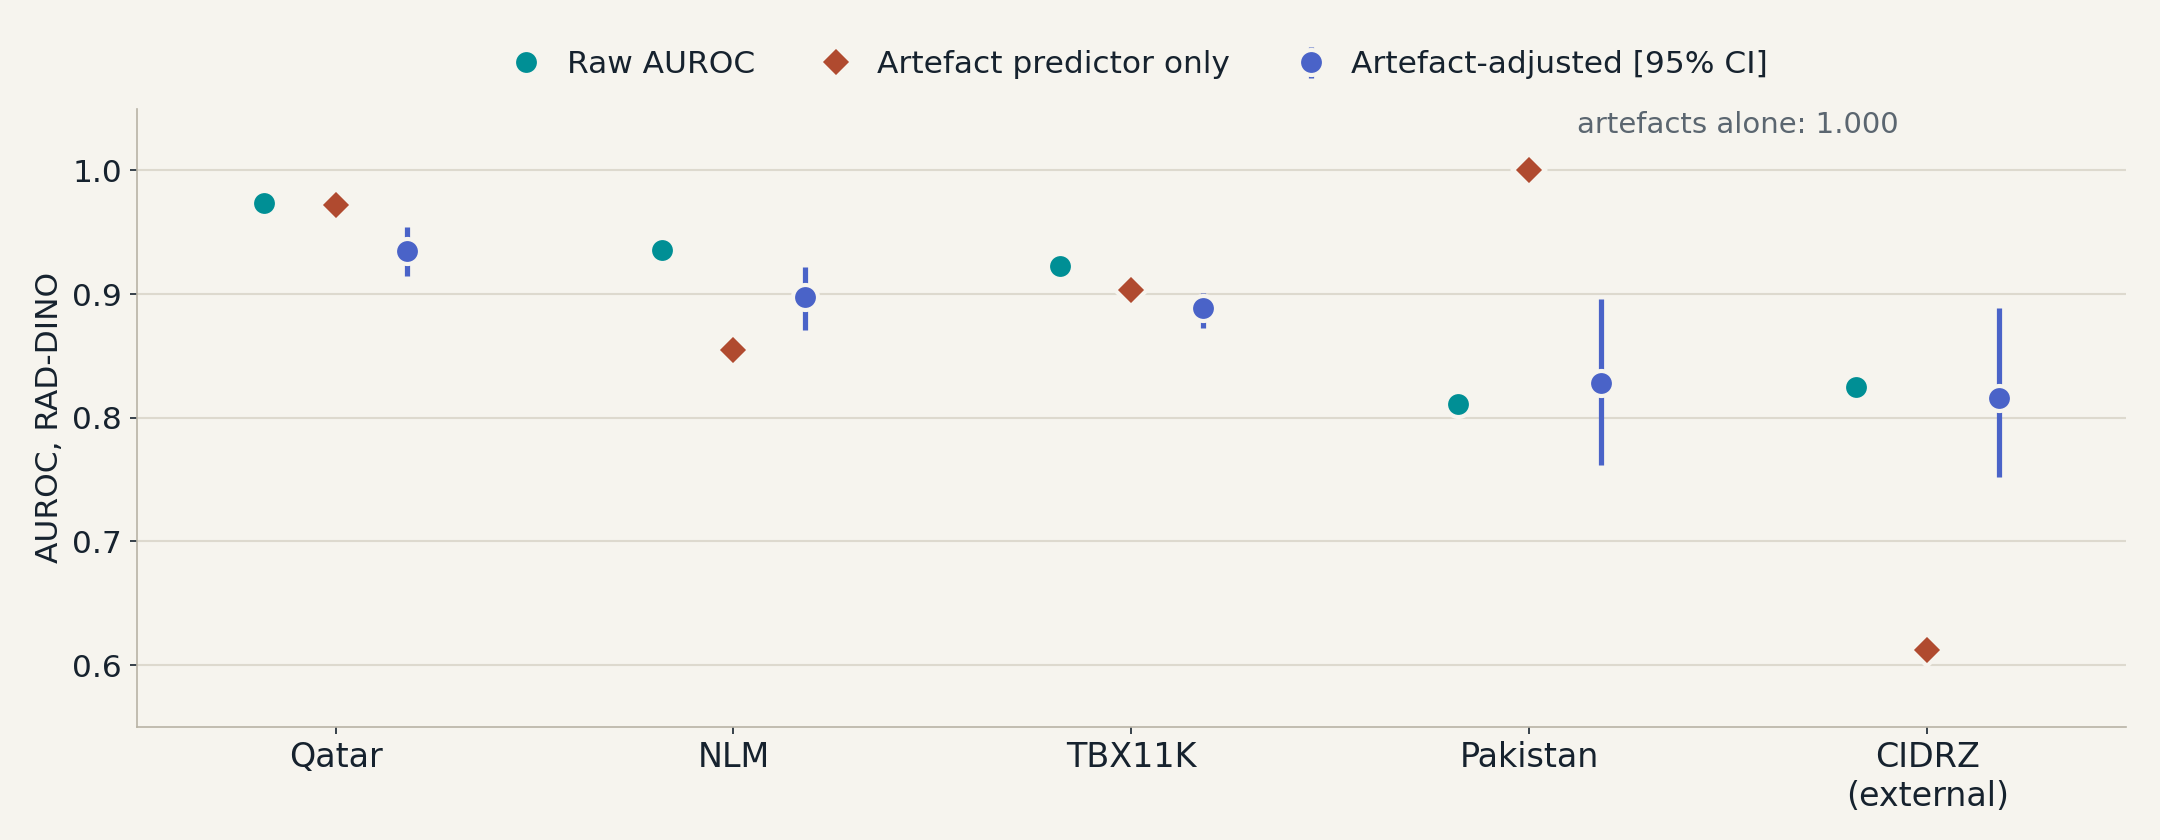
\includegraphics[width=.95\linewidth]{fig_artefact_dots.png}
\caption{RAD-DINO raw AUROC, artefact-predictor-only AUROC and artefact-adjusted AUROC with 95\% CIs. Where the artefact predictor (red diamond) is close to the raw score (teal dot), the raw score is largely explained by artefacts: Qatar and, extremely, Pakistan. On CIDRZ the artefact predictor is near chance and the adjusted score barely moves.}\end{figure}
On CIDRZ, where artefacts are weakly predictive (0.61), adjustment changes AUROC by 0.009: the 0.8 AUROC is not an artefact effect. On Qatar, NLM and TBX11K the drop is 0.03--0.04, so the models add signal beyond the artefact predictor, but the artefact-only baselines are strong (0.86--0.97), so raw AUROCs there overstate generalization. On Pakistan the artefact-only AUROC is 1.000 and only 1\% of pairs survive stratification: the label is confounded with the source, the adjusted number is not identifiable, and Pakistan should not be used as evidence of generalization.

\section{Results: multimodal fusion on CIDRZ}
Table~\ref{tab:fusion} and Figure~\ref{fig:fusion} use the final image expert: the corrected RAD-DINO and tuned ViT, five seeds each, ensembled, trained on all four source corpora and never on CIDRZ (image alone AUROC 0.827; 0.824 for RAD-DINO alone). The text and audio experts and the fusion layers are fit in cross-validation on CIDRZ.
\begin{figure}[H]\centering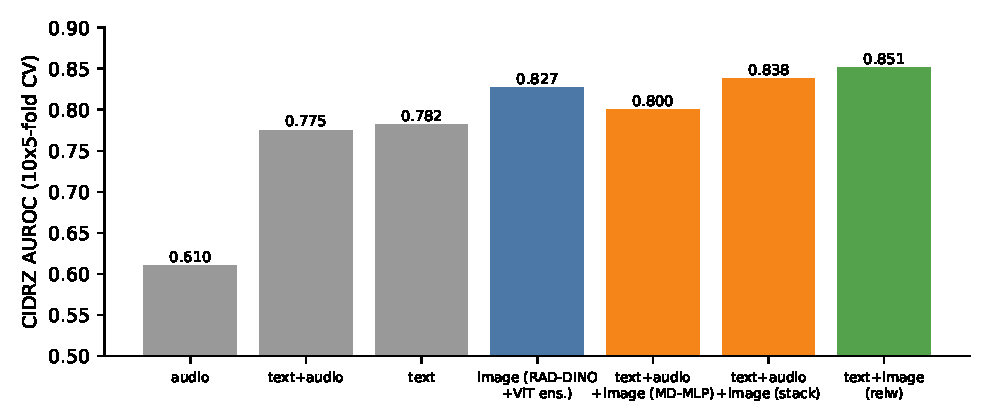
\includegraphics[width=.8\linewidth]{fig_fusion.pdf}
\caption{CIDRZ AUROC for single modalities and fusion arms (RAD-DINO + ViT ensemble expert).}\label{fig:fusion}\end{figure}
\begin{table}[H]\centering\small
\begin{tabular}{lcc}\toprule
Arm & AUROC & $\Delta$ vs same method without image [95\% CI]\\\midrule
audio & 0.610 & --\\
text & 0.782 & --\\
text + audio (stack) & 0.775 & --\\
image alone & 0.827 & --\\
text + image, stack / relw / concat & 0.844 / \textbf{0.851} / 0.843 & --\\
text + audio + image, stack & 0.838 & $+0.058$ [$+0.013,+0.103$]\\
text + audio + image, relw & 0.847 & $+0.060$ [$+0.021,+0.098$]\\
text + audio + image, concat & 0.816 & $+0.045$ [$+0.017,+0.073$]\\
text + audio + image, MD-MLP & 0.800 & $+0.051$ [$+0.022,+0.081$]\\\bottomrule
\end{tabular}\caption{CIDRZ fusion (10$\times$ repeated 5-fold CV).}\label{tab:fusion}\end{table}
\begin{itemize}
\item Adding the image expert improves text + audio by $+0.045$ to $+0.060$ AUROC for every fusion method, with 95\% CIs excluding 0. Reliability-weighted text + image is best (0.851 vs text 0.782).
\item Audio contributes nothing: text + audio (0.775) is not better than text (0.782), and text + image beats text + audio + image.
\item The gain depends on expert quality: with the plain ERM image expert (0.760) the text + audio + image gain is $+0.026$ [$-0.015,+0.062$], not significant. With the corrected RAD-DINO (0.824) and ViT/RAD-DINO ensemble (0.827) experts it is $+0.062$ and $+0.060$. (The earlier RAD-DINO result, $+0.052$, came from the pre-fix expert.)
\item MD-MLP trained with modality dropout degrades gracefully when audio is missing (0.825) but drops to about 0.74--0.75 when the text or image is missing.
\item CIDRZ appears capped near 0.80--0.85 AUROC (the 0.01 higher image expert barely moves fusion) for these experts; with 60 positives the CIs are wide ($\pm$0.04--0.05).
\end{itemize}

\section{Calibration, WHO operating points and local recalibration}
Training used source-balanced cells, so logits are not prevalence-calibrated. Every expert is over-confident on held-out corpora (logistic calibration slope 0.2--0.6; ECE 0.04--0.24 on public corpora and 0.49 on CIDRZ for RAD-DINO, 0.27 for ViT, 0.57 for ERM). On CIDRZ the raw Brier score (0.22--0.45) is worse than the constant-prevalence predictor (0.138) although AUROC is $\approx$0.8: ranking transfers, probabilities do not. The 90\%-sensitivity threshold chosen on held-in validation data gives target sensitivity 0.54--0.77 and specificity 0.76--1.00 (RAD-DINO, CIDRZ: 0.71/0.76), i.e.\ the source-trained threshold is too conservative on the new site.
\paragraph{Definitions and worked examples.}\label{sec:calib-defs} \emph{Expected calibration error} (ECE) groups predictions into bins by stated probability; in each bin the gap is the absolute difference between the mean stated probability and the fraction that truly had TB, and ECE averages the gaps weighted by the number of images per bin (0 is ideal). It says nothing about ranking: a model can have an excellent AUROC and a poor ECE, which is what happens on CIDRZ. The \emph{Brier score} is the mean squared error of the predicted probabilities (lower is better); the \emph{calibration slope} is the slope of a logistic regression of the labels on the logit score (ideal 1; below 1 means over-confident). Illustrative numbers, not our data:
\begin{table}[H]\centering\small
\begin{tabular}{lccc}\toprule
Model says & Images & Truly TB & Gap\\\midrule
about 20\% & 400 & 10\% & 0.10\\
about 50\% & 300 & 25\% & 0.25\\
about 70\% & 200 & 40\% & 0.30\\
about 90\% & 100 & 60\% & 0.30\\\bottomrule
\end{tabular}\end{table}
ECE $=(400\times0.10+300\times0.25+200\times0.30+100\times0.30)/1000=0.205$.

\emph{Platt scaling} maps a raw score $s$ to a probability with a two-parameter logistic map,
\[P(\mathrm{TB}\mid s)=\frac{1}{1+\exp\!\bigl(-(a\,s+b)\bigr)},\]
fitted by logistic regression of the true labels on the scores of a small labelled sample from the new site. The slope $a$ corrects over-confidence and the intercept $b$ corrects the TB rate at the new site; intercept-only recalibration fixes just $b$ (the prior). The map is monotone, so ranking, and hence AUROC, is unchanged.
\begin{figure}[H]\centering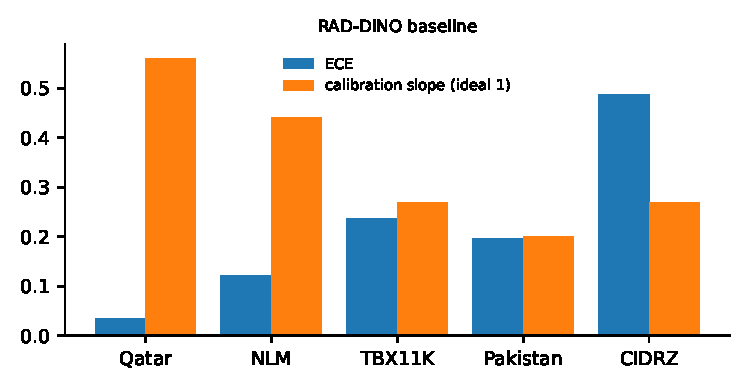
\includegraphics[width=.6\linewidth]{fig_calib.pdf}
\caption{Calibration of the final RAD-DINO model on each held-out corpus.}\end{figure}
\begin{table}[H]\centering\small
\begin{tabular}{lccccc}\toprule
RAD-DINO (5 seeds) & Qatar & NLM & TBX11K & Pakistan & CIDRZ\\\midrule
ECE & .035 & .121 & .237 & .197 & .487\\
Slope & .56 & .44 & .27 & .20 & .27\\
Transfer sens./spec. & .75/1.00 & .56/.98 & .55/.96 & .67/.83 & .71/.76\\\bottomrule
\end{tabular}\caption{Calibration of the final RAD-DINO model.}\end{table}

\paragraph{WHO triage profile and local recalibration.} The WHO target product profile for a triage test is at least 90\% sensitivity and at least 70\% specificity. We ask whether a small labelled local sample ($k=25$--$400$ cases) can adapt the model: local Platt scaling, intercept-only recalibration, and a local 90\%-sensitivity threshold, repeated 300 times (\texttt{local\_recalibration.py}). Findings:
\begin{itemize}
\item \emph{Calibration is repairable.} For RAD-DINO on CIDRZ, ECE falls from 0.50 to 0.11 (intercept only) and 0.06--0.08 (Platt) with 25--200 labelled cases; ViT from 0.25 to 0.07--0.09.
\item \emph{Discrimination is not.} On CIDRZ the oracle operating points are sensitivity 0.82 at 70\% specificity, or specificity 0.50 at 90\% sensitivity (RAD-DINO; ViT 0.78 and 0.39). No threshold meets the profile; the probability that a locally chosen threshold does is 0.00 for every $k$. With a 50-case local sample the local 90\%-sensitivity threshold delivers 0.80 sensitivity and 0.61 specificity.
\item \emph{On public corpora the profile is reachable} (oracle 0.94 sens.\ at 77\% specificity on TBX11K, 0.97/0.96 on Qatar), but a local threshold from 50--200 cases meets it only 10--40\% of the time because the target sensitivity is estimated from few positives; Pakistan (oracle specificity 0.25 at 90\% sensitivity) never does.
\end{itemize}
A model can therefore be well calibrated at a site and still fall short of the clinical target; local labelled data fix probabilities and thresholds, not ranking quality. The fused text + image score reaches AUROC 0.85 on CIDRZ; we did not evaluate its operating points against the profile.

\paragraph{Is the CIDRZ shortfall a matter of cohort size?}\label{sec:why-cidrz} In part. With 60 positives the oracle operating points are imprecise (Table~\ref{tab:ceilboot}, \texttt{ceiling\_bootstrap.py}): for RAD-DINO the 95\% bootstrap interval is 0.69--0.90 for sensitivity at 70\% specificity and 0.33--0.71 for specificity at 90\% sensitivity, so the upper ends just touch the profile. But only 2.6\% of resamples meet both targets (1.1\% for ViT); the point estimates, which reflect an AUROC of about 0.8, are well short of them, and more positives would narrow the interval around those estimates rather than move them. Whether the true performance at this site is a little higher cannot be settled with 60 positives. Differences in reference standard (microbiological here, radiologist reading on VinDr-CXR), case mix and image acquisition may also contribute; with two external cohorts they cannot be separated from site effects.
\begin{table}[H]\centering\small
\begin{tabular}{lccc}\toprule
CIDRZ (364 images, 60 positives) & sens.\ at 70\% spec.\ [95\% CI] & spec.\ at 90\% sens.\ [95\% CI] & P(both)\\\midrule
RAD-DINO & 0.82 [0.69, 0.90] & 0.50 [0.33, 0.71] & 0.026\\
RAD-DINO + MixStyle & 0.80 [0.70, 0.90] & 0.42 [0.26, 0.72] & 0.028\\
ViT (tuned) & 0.78 [0.66, 0.88] & 0.39 [0.17, 0.65] & 0.011\\\bottomrule
\end{tabular}\caption{Bootstrap (4000 resamples of the 364 images) of the oracle WHO-profile operating points on seed-averaged scores. P(both): share of resamples in which sensitivity $\ge$0.90 and specificity $\ge$0.70 are both reached.}\label{tab:ceilboot}\end{table}

\section{Second external cohort: VinDr-CXR}\label{sec:vindr}
\paragraph{Cohort, labels and sampling.} VinDr-CXR 1.0.0 (PhysioNet, credentialed access) has 18\,000 postero-anterior radiographs (15\,000 train, 3\,000 test) annotated by radiologists for 28 findings. TB-positive is the radiologists' ``Tuberculosis'' finding: at least two of three reads on the training split (482 images; 247 unanimous; 268 images with exactly one TB read are excluded as ambiguous) and the consensus label on the test split (164). These are image read-outs, not microbiological confirmation. We downloaded all 646 positives and 1\,500 sampled TB-free images (1\,000 train, 500 test; half ``No finding'', half other findings), 2\,146 DICOMs (12\% of the release). Because the sample is enriched (30.1\% TB; the release has about 3.6\% among labelled-TB and TB-free images) every image carries the inverse of its sampling probability (21.2 and 7.3 for training ``No finding''/other, 8.2 and 3.1 for the test split, 1 for positives), and all metrics below are weighted unless stated; unweighted AUROCs are about 0.01 lower. MONOCHROME1 DICOMs (25\%) were inverted, JPEG\,2000 decoded, and the same min--max/resize and lung masking as the other corpora applied (mask area 0.41, 2 failures). The eight tuned configurations of Table~\ref{tab:loco} were retrained with VinDr as the held-out target (five seeds, four public sources, same held-in split), and their CIDRZ AUROCs reproduce Table~\ref{tab:loco} to three decimals for the six non-RAD-DINO configurations.
\begin{table}[H]\centering\footnotesize\setlength{\tabcolsep}{3.6pt}
\begin{tabular}{lcccccc}\toprule
Method (5 seeds) & per-seed AUROC & seed-avg [95\% CI] & vs ``No finding'' & vs other findings & $\Delta$ vs ViT [95\% CI]\\\midrule
RAD-DINO + MixStyle & .917$\pm$.018 & .935 [.924,.947] & .950 & .894 & $+.048$ [.034,.064]\\
RAD-DINO & .903$\pm$.013 & .919 [.905,.932] & .930 & .888 & $+.032$ [.018,.049]\\
ViT (tuned) & .870$\pm$.016 & .887 [.870,.903] & .899 & .854 & --\\
ResNet50 & .864$\pm$.019 & .882 [.865,.897] & .894 & .844 & $-.005$ [$-$.019,.009]\\
ViT sbal, whole image & .848$\pm$.027 & .872 [.853,.891] & .893 & .809 & $-.015$ [$-$.031,.002]\\
ViT + MixStyle & .846$\pm$.020 & .864 [.846,.882] & .874 & .837 & $-.023$ [$-$.028,$-$.016]\\
ViT ERM, whole image & .837$\pm$.032 & .866 [.846,.885] & .882 & .813 & $-.021$ [$-$.038,$-$.004]\\
xrv-DenseNet121 & .825$\pm$.015 & .836 [.814,.854] & .840 & .822 & $-.051$ [$-$.068,$-$.036]\\\bottomrule
\end{tabular}\caption{VinDr-CXR, weighted AUROC. CIs and paired differences use a bootstrap that resamples within split $\times$ label $\times$ stratum cells (\texttt{results/vindr\_eval.md}, \texttt{results/vindr\_paired.md}).}\label{tab:vindr}\end{table}
\begin{itemize}
\item \textbf{The foundation-model advantage is confirmed externally.} On CIDRZ no backbone differed; on VinDr RAD-DINO beats tuned ViT by $+0.032$ and RAD-DINO + MixStyle by $+0.048$ with CIs that exclude 0, ResNet50 is equal to ViT, and xrv-DenseNet is lowest. MixStyle helps RAD-DINO ($+0.016$) but hurts ViT ($-0.023$), so it remains an unreliable gain.
\item \textbf{Hard negatives matter.} RAD-DINO AUROC is 0.930 against ``No finding'' negatives but 0.888 against negatives with other findings; it is 0.932 on training-split rows (three-reader majority) and 0.882 on test-split rows (consensus). It scores positives without an active-pattern finding (no cavity, infiltration, consolidation or nodule flagged; 403 of 646) as well as those with one (0.906 vs 0.914).
\item \textbf{Artefacts are not negligible but do not explain the score.} A silhouette/border artefact predictor reaches weighted AUROC 0.72 (trained on the sources) or 0.79 (cross-validated inside VinDr), well above its 0.61 on CIDRZ. Stratifying on it (10 bins, 8\% of pairs kept) moves RAD-DINO from 0.919 to 0.899 (MixStyle 0.935 $\rightarrow$ 0.916; ViT 0.887 $\rightarrow$ 0.846), and RAD-DINO adds $+0.144$ AUROC over the artefact score in cross-validation.
\end{itemize}
\begin{table}[H]\centering\footnotesize\setlength{\tabcolsep}{3.6pt}
\begin{tabular}{lcccccc}\toprule
Method & oracle sens. & oracle spec. & transfer sens./spec. & PPV & ECE & slope\\\midrule
RAD-DINO + MixStyle & 0.95 & 0.79 & .64/.98 & 0.52 & .212 & .53\\
RAD-DINO & 0.91 & 0.73 & .59/.97 & 0.44 & .248 & .47\\
ViT (tuned) & 0.88 & 0.65 & .55/.95 & 0.30 & .130 & .49\\
ResNet50 & 0.87 & 0.65 & .57/.94 & 0.26 & .153 & .52\\
xrv-DenseNet121 & 0.79 & 0.52 & .60/.90 & 0.18 & .282 & .67\\\bottomrule
\end{tabular}\caption{VinDr-CXR operating points against the WHO triage profile (sensitivity $\ge$90\%, specificity $\ge$70\%) and calibration of the seed-averaged weighted scores. Oracle sens.: sensitivity at 70\% specificity; oracle spec.: specificity at 90\% sensitivity. ``Transfer'' is the threshold giving 90\% sensitivity on held-in validation data. PPV is at 3.6\% prevalence; ECE and slope are for the raw probabilities.}\label{tab:vindrwho}\end{table}
\paragraph{WHO profile and calibration.} With an oracle threshold the two RAD-DINO models reach the profile on VinDr (sensitivity 0.91 at 70\% specificity, specificity 0.73 at 90\% sensitivity), which no model did on CIDRZ (0.82 and 0.50). The deployable zero-label threshold does not: the held-in 90\%-sensitivity threshold delivers sensitivity 0.59--0.64 at specificity 0.97--0.98 (too conservative, as on CIDRZ). A local threshold set on $k=50$--$400$ labelled cases meets the profile with probability 0.04--0.17 for RAD-DINO and 0.19--0.51 for RAD-DINO + MixStyle, and 0.00 for the other backbones. Raw probabilities are badly calibrated at the true prevalence (ECE 0.13--0.28, slope about 0.5, intercept $-2.8$ to $-4.0$); local Platt scaling with $k=50$--$400$ cases, fitted with the sampling weights, brings ECE to 0.017--0.008 (intercept-only 0.023--0.015) and Brier from 0.19 to 0.02, again repairing calibration but not discrimination. \emph{These operating-point results are optimistic}: the WHO profile is defined against a microbiological reference, whereas VinDr's reference is radiologist reading, which an image model trained on radiologist-labelled corpora can partly imitate; CIDRZ, with a microbiological reference, is the stricter test and fails it.

\section{Limitations}
\begin{itemize}
\item There are two documented external cohorts. CIDRZ has a microbiological reference but only 60 positives (CIs $\pm$0.04--0.07); VinDr-CXR has 646 positives but its TB labels are radiologist read-outs (a three-reader majority on the training split, a consensus on the test split), so it measures agreement with readers, and its evaluation sample is enriched for TB and re-weighted. An additional public cohort (India CXR set) was rejected because its labels are ``Abnormal'' rather than TB (\texttt{results/tb\_multi\_india\_report.md}); PadChest and NIAID TB Portals were not obtained.
\item VinDr's ``Tuberculosis'' label may include old or inactive disease, which the source corpora label differently; fused text/audio experts do not apply to VinDr; one within-VinDr near-duplicate was kept; RAD-DINO re-training is not bit-reproducible (its CIDRZ AUROC moved by $-0.019$ and $-0.008$ for the two RAD-DINO variants between the main and the VinDr runs, within the seed standard deviation; the other six configurations reproduced to three decimals).
\item Tuning used seed 0 on four folds, two of them artefact-prone; gains were small. The 448\,px arm has two seeds. Lesion supervision and DG losses were not re-run with the tuned configuration or five seeds.
\item Qatar and Pakistan labels are partly predictable from artefacts; artefact adjustment is a bound, not a causal fix, and is not identifiable on Pakistan.
\item Deduplication does not cover heavy crops or flips. Calibration and recalibration were assessed on image-expert scores, not on fused probabilities. The UAR column of the fusion tables thresholds raw scores at 0 and is not meaningful for relw; use AUROC.
\end{itemize}

\section{Next steps}
\begin{itemize}
\item Add a larger cohort with microbiological labels (PadChest or NIAID TB Portals; the Kaggle PadChest sample has only 24 images and no TB label, so it cannot serve as a test set).
\item Spot-check labels and count positives before trusting any new target, then re-run the audit, the artefact adjustment and the recalibration on it.
\item Evaluate the operating points of the fused text + image score against the WHO profile, and run VinDr-CXR at 448\,px.
\end{itemize}

\section{Conclusions and recommendations}
\begin{enumerate}
\item Audit before training: corpus identity and silhouette/border shortcuts explain much of the apparent performance on some corpora. Report LOCO, not pooled, results, with artefact-only and artefact-stratified AUROC alongside.
\item Use a CXR-pretrained backbone (RAD-DINO) with lung masking and strong augmentation: LOCO mean 0.898 against 0.867 for tuned ViT. On the external CIDRZ cohort (60 positives) all backbones are indistinguishable (0.77--0.81), but on VinDr-CXR (646 positives) RAD-DINO leads tuned ViT by $+0.03$ to $+0.05$ (paired CIs exclude 0).
\item Classical DG losses and MixStyle do not help beyond source-balanced sampling.
\item For multimodal TB screening, fuse a source-trained CXR expert with the text/clinical expert (reliability-weighted: 0.851 vs 0.782); audio did not help in this cohort.
\item Recalibrate per site: a few dozen labelled local cases fix probabilities (ECE 0.50 $\rightarrow$ 0.07) but not discrimination; on CIDRZ no model meets the WHO triage profile (90\% sensitivity, 70\% specificity), and on VinDr only the RAD-DINO models reach it, with an oracle threshold and radiologist labels.
\item Follow the audit protocol in Appendix~\ref{app:audit} and say which numbers were superseded after any bug fix.
\end{enumerate}

\appendix
\section{Cross-corpus audit protocol}\label{app:audit}
Each item is tied to a measured result in this report (full version: \texttt{results/audit\_protocol.md}).
\begin{enumerate}[leftmargin=*]
\item \textbf{Deduplicate across corpora before splitting}, with a positive control (400 planted TBX11K copies recovered).
\item \textbf{Evaluate leave-one-corpus-out}, not random splits: rankings change by corpus (ViT ERM 0.87 on Pakistan, 0.69 on TBX11K).
\item \textbf{Run source-prediction and artefact-only controls}: artefact-only AUROC 0.64--1.00 within corpus.
\item \textbf{Report artefact-stratified AUROC beside raw AUROC} (RAD-DINO Qatar 0.974 $\rightarrow$ 0.935; CIDRZ 0.825 $\rightarrow$ 0.816).
\item \textbf{Declare a corpus non-identifiable when artefacts predict the label} (Pakistan: 1.000, 1\% of pairs kept) and do not cite it as evidence of generalization.
\item \textbf{Validate the labels of every added cohort} (the India set was ``Abnormal'', not TB; rejected; VinDr's labels are radiologist reads and are reported as such, with sampling weights for the enriched sample).
\item \textbf{Fix the tuning protocol before looking at the external target}; report alternative selections.
\item \textbf{Use $\ge$5 seeds and paired bootstrap CIs}; claim only what excludes zero (all CIDRZ differences include zero).
\item \textbf{Check checkpoint restore and train/eval parity} (a partial restore moved ResNet50 AUROC by 0.026).
\item \textbf{Check resolution after the artefact audit} (448\,px: $+0.03$--0.04 on NLM/TBX11K, $+0.004$ on CIDRZ).
\item \textbf{Report calibration separately from discrimination} (CIDRZ ECE 0.49 $\rightarrow$ 0.07 after local Platt).
\item \textbf{Report against the clinical target with an oracle threshold} (WHO triage: 90\%/70\%; CIDRZ ceiling 0.82 sens.\ at 70\% spec.; VinDr RAD-DINO 0.91, with radiologist labels).
\item \textbf{Keep pre-fix and post-fix runs in separate tables and say which numbers were superseded.}
\end{enumerate}

\section{Glossary}\label{app:glossary}
\begin{description}[leftmargin=2.2cm,labelwidth=2cm,itemsep=2pt,font=\bfseries]
\item[TB] Tuberculosis, a bacterial lung infection; on an X-ray it can show as opacities, nodules or cavities.
\item[CXR] Chest X-ray: a cheap, fast image that AI reads to flag who needs a laboratory test.
\item[Prevalence] Share of people in a dataset who have TB (8\% to 83\% across our corpora).
\item[Sensitivity, specificity] Share of TB cases the model flags; share of non-TB people it clears. Both depend on the threshold. PPV (positive predictive value) is the share of flagged people who truly have TB and depends on prevalence.
\item[AUROC] Area under the ROC (receiver operating characteristic) curve: the chance that a random TB case scores above a random non-TB case; 0.5 is a coin flip, 1.0 is perfect. It does not depend on a threshold.
\item[WHO TPP] WHO target product profile: a triage test should reach at least 90\% sensitivity and 70\% specificity.
\item[Backbone] The pretrained network that turns an image into features; \textbf{fine-tuning} keeps training it on TB images, here updating only its last blocks.
\item[ViT] Vision Transformer, an image model that reads a picture as a grid of patches; here pretrained on everyday photos.
\item[RAD-DINO] A self-supervised vision model from Microsoft pretrained on chest X-rays.
\item[xrv] TorchXRayVision: a DenseNet121 pretrained on many chest X-ray sets.
\item[Domain shift, LOCO] Sites differ in scanners, patients and labelling. Leave-one-corpus-out trains on some corpora and tests on the held-out one.
\item[Seed, sd, CI] A seed fixes the random start of training; sd is the standard deviation across seeds; a bootstrap confidence interval (CI, 95\% here) shows what is noise. A difference whose CI includes 0 is not a claim that one method is better.
\item[ERM] Empirical risk minimization: plain training with no extra tricks.
\item[Calibration, ECE, Brier] Whether predicted probabilities match reality; see Section~\ref{sec:calib-defs}.
\item[Platt scaling] Recalibration by a small logistic map from scores to probabilities.
\item[Artefact, shortcut] A cue that predicts the label but is not disease: scanner marks, borders, burnt-in text, image shape.
\item[Lung mask] Black out everything outside the lungs so the model cannot use those cues.
\item[sbal, dstd] Source-balanced sampling; per-domain feature standardization.
\item[DG] Domain generalization: MixStyle, GroupDRO, V-REx, CORAL, DANN (Section~\ref{sec:methods}).
\item[relw, MD-MLP] Reliability-weighted late fusion; a fusion MLP trained with modality dropout.
\item[Deduplication] Removing near-identical images shared across corpora; otherwise test images leak into training.
\item[NLM] US National Library of Medicine: the Montgomery and Shenzhen sets.
\item[TBX11K] A large public TB chest X-ray set that includes lesion boxes.
\item[Pakistan] The Mendeley (v3) TB set; mostly TB, small JPEGs.
\item[CIDRZ] Centre for Infectious Disease Research in Zambia, released as the Google Health AI cohort with clinical text, cough audio and chest X-rays; our first external cohort.
\item[VinDr-CXR] A Vietnamese chest X-ray set on PhysioNet with radiologist-labelled findings; our second external cohort.
\end{description}

\section*{Reproducibility}\sloppy
Code in \texttt{datasets/tb\_multi/} (\texttt{standardize}, \texttt{dedup}, \texttt{embed}, \texttt{masks}, \texttt{shortcut\_audit}, \texttt{loco\_train}, \texttt{summarize\_loco}, \texttt{fusion\_study}, \texttt{calibration}, \texttt{download\_vindr}, \texttt{dedup\_external}, \texttt{vindr\_report}, \texttt{vindr\_paired}, \texttt{ceiling\_bootstrap}); outputs in \texttt{results/} (\texttt{loco\_final/*.json}, \texttt{loco\_final\_summary.md}, \texttt{loco\_448/}, \texttt{tuning\_summary.md}, \texttt{artefact\_adjusted.md}, \texttt{local\_recalibration.md}, \texttt{fusion\_study\_corrected.md}, \texttt{calibration\_final.md}, \texttt{audit\_protocol.md}, \texttt{loco\_vindr/*.json}, \texttt{vindr\_eval.md}, \texttt{vindr\_paired.md}, \texttt{vindr\_selection.csv}, \texttt{ceiling\_bootstrap.md}). Dependencies: \texttt{pip install ".[tb\_multi]"} (CUDA torch installed separately).
\end{document}
